

\subsection{Controlled ablation on the CMU20 benchmark}

\begin{figure}
    \centering
    
\includegraphics[width=0.95\linewidth]{images/figure2_combined_panelabc.png}
  \caption{\textbf{Ablation analysis on the CMU20 benchmark across four LLM backends.} 
  (a) Comparison of best energy across different methods in all 20 cases - Heuristic, Random, AdsMind (M: use MACE-MP-0-small for force field), Adsorb-Agent (E: use EquiformerV2 for force field).
  (b) Trapezoid plots of energy error ($\Delta E = E_{\mathrm{variant}} - E_{\mathrm{Full}}$) for each ablation setting. Each variant (1-Shot, w/o Slip, w/o Forbid, w/o Term) is evaluated on all 20 cases across four LLM backends (393 successful runs out of 400). Positive values indicate higher (worse) adsorption energy than the Full variant; the dashed line at $\Delta E = 0$ marks parity. 
  (b) Radar chart comparing the Full variant against ablated variants across four performance dimensions: Success Rate (fraction of runs reaching a valid low-energy configuration), Energy Accuracy (fraction within 0.01~eV of the best observed energy), Backend Robustness (inverse of cross-backend energy spread), and Cross-LLM Agreement (consistency of predicted site across backends). Higher values indicate better performance; the Full variant (blue) provides the strongest aggregate balance across the four metrics, while individual ablations can improve selected dimensions.}
  \label{fig:cmu20_ablation}
\end{figure}

We evaluated the agent on the completed 20-case CMU benchmark, spanning H, NNH, OH, CH$_2$CH$_2$OH, OCHCH$_3$, and ONN(CH$_3$)$_2$ adsorption across increasingly difficult intermetallic and monometallic surfaces.
For each case, we executed five runtime variants under a fixed MACE-MP-0 small CPU backend~\cite{batatia2023foundation}: Full, without Slip (w/o Slip), without Forbid (w/o Forbid), without Term (w/o Term), and 1-Shot.
Here w/o Slip removes slip-conditioned guidance together with its associated FORBID constraint. w/o Forbid keeps slip detection and history but removes the explicit ``do not retry this site'' instruction. w/o Term disables convergence-based early stopping, and 1-Shot reduces the total budget to a single attempt.
The complete 20$\times$5 matrix was executed independently on four LLM backends---Gemini~2.5~Pro, Grok-4, GPT-5.4, and Claude~Sonnet~4.6---yielding 393 successful runs out of 400 attempts.
Figure~\ref{fig:cmu20_ablation} summarizes the ablation results.

\paragraph{Completion status and success rates.}
The newly completed cases (03, 06, 07, 08, 11) close the CMU benchmark gap across all five variants.
The Full, w/o Slip, w/o Forbid, and w/o Term variants achieve 100\% success (320/320 runs across CMU20).

\paragraph{1-Shot failure mode: chemical dissociation.}
In contrast, the 1-Shot variant exhibits a distinct failure mode not seen in iterative variants.
Case~06 fails on all four backends and case~08 fails on three of four (Grok-4, GPT-5.4, and Claude; Gemini's single attempt matches its Full energy), yielding 73/80 successful 1-Shot runs (91.3\%).
These failures are not external system errors; in each case the relaxation completes, but the final structure is rejected because \texttt{is\_dissociated=True} with \texttt{dissociation\_count=1} and no valid best adsorption energy.
This is a natural chemical outcome rather than a planning failure.

\paragraph{Cross-backend consistency.}
To quantify agreement across LLM backends, we define the four-backend range as the max-min energy spread across Gemini, Grok-4, GPT-5.4, and Claude for a given case.
Across CMU20, the mean four-backend range is 0.195~eV (median 0.037~eV), with 7/20 cases agreeing within 0.01~eV and 11/20 within 0.05~eV.
The largest disagreement occurs on case~08 (Ru$_3$Mo + NNH), where GPT-5.4 reaches $-7.191$~eV, Claude reaches $-6.869$~eV, and Gemini/Grok-4 remain at $-6.414$~eV.
Thus, the Full agent is reliable on CMU20, while backend agreement remains case-dependent rather than universal.

Table~\ref{tab:key-evaluation-metrics} reports the formal statistical evaluation across all four backends. Cases with censored 1-Shot attempts due to natural dissociation or reaction failures are retained in the aggregate statistics but flagged in the per-case audit. The Supporting Information provides full per-backend energy matrices, success rates, and failure audits.

\begin{table}[t]
\centering
\caption{Key evaluation metrics across all four backends on the 20-case CMU benchmark.}
\label{tab:key-evaluation-metrics}
\begin{tabular}{p{3.3cm}p{1.3cm}p{1.8cm}p{1.8cm}p{1.8cm}p{1.8cm}p{1.0cm}}
\toprule
Metric & Target & Gemini & Grok-4 & GPT-5.4 & Claude & Met \\
\midrule
Friedman $p$~\cite{friedman1937use} & $< 0.05$ & 1.98e-07 & 2.56e-08 & 1.23e-03 & 2.61e-05 & 4/4 \\
H$_1$ support & $\geq$75\% & 6/13 (46\%) & 5/12 (42\%) & 6/13 (46\%) & 8/13 (62\%) & --- \\
BH $p$ (1-Shot)~\cite{benjamini1995controlling} & $< 0.05$ & 0.0431 & 0.2123 & 0.1763 & 0.0355 & 2/4 \\
Backend conv. & Lower & \multicolumn{4}{p{7.2cm}}{Full mean range 0.195~eV vs.\ 0.473~eV 1-shot; 2.42$\times$ reduction.} & Yes \\
\bottomrule
\end{tabular}
\end{table}

The Friedman test~\cite{friedman1937use} is highly significant on all four backends: Gemini ($p = 1.98 \times 10^{-7}$), Grok-4 ($p = 2.56 \times 10^{-8}$), GPT-5.4 ($p = 1.23 \times 10^{-3}$), and Claude ($p = 2.61 \times 10^{-5}$).
Pairwise Wilcoxon tests~\cite{wilcoxon1945individual} confirm that the full agent significantly outperforms the 1-shot baseline after BH correction~\cite{benjamini1995controlling} on Gemini and Claude (Gemini BH~$p = 0.0431$, Claude BH~$p = 0.0355$), but not on Grok-4 (BH~$p = 0.2123$) or GPT-5.4 (BH~$p = 0.1763$).
Although the directional H$_1$ support criterion does not reach the pre-specified 75\% threshold on any backend, the rank-based Friedman tests remain significant on all four backends.
This indicates that the closed-loop gain is statistically robust but heterogeneous across cases rather than uniformly positive on every benchmark item.

\paragraph{The closed-loop gain is large and backend-dependent.}
The mean full-versus-single-shot improvement varies from 0.108~eV (GPT-5.4) to 0.297~eV (Grok-4), with Gemini at 0.296~eV and Claude at 0.163~eV.
The largest per-case improvements occur on complex surfaces: case~20 shows 1-shot deficits exceeding 1.0~eV on both Gemini and Grok-4, while case~15 consistently degrades under single-shot across all four backends and case~12 degrades on three of four (Gemini, Grok-4, Claude; tied on GPT-5.4).
GPT-5.4 shows the smallest mean improvement, consistent with a stronger one-shot planner that leaves less room for iterative recovery; however, it still gains 0.426~eV on case~02 and 0.549~eV on case~17.

\paragraph{Ablated variants occasionally outperform full on edge cases.}
While the full agent achieves superior aggregate performance across CMU20, case-level analysis reveals instances where ablations find lower energies (e.g., case~18: w/o Slip $-$0.491~eV vs Full on GPT-5.4).
These instances are edge cases where early attempts happen to locate favorable configurations; the FORBID constraint then over-prunes the remaining search space, preventing exploration of potentially better solutions.
This behavior is a predictable trade-off: guardrails improve reliability and cross-backend consistency across the benchmark, but impose a small expected cost when the initial search trajectory is already a favorable low-energy basin.
The aggregate statistics confirm this interpretation: w/o Forbid and w/o Term both trend toward improving over full on GPT-5.4 (BH~$p = 0.084$), yet the full variant maintains higher success rates and tighter backend convergence overall (Table~\ref{tab:key-evaluation-metrics}).

\paragraph{Termination balances compute cost against marginal chemistry gains.}
Disabling termination improves energy modestly on some backends (e.g., Grok-4 mean $-$0.047~eV) but increases token consumption 2--6$\times$; the default termination criterion therefore captures most attainable improvement at minimal cost.

\paragraph{Iteration convergence.}
Rapid iteration convergence underlies this efficiency: iteration~2 captures 58--80\% of the total improvement and iteration~3 captures 80--87\%, after which returns diminish sharply (Figure~\ref{fig:cmu20_convergence}a). Most closed-loop value is extracted within 2--3 iterations, making the default budget near-optimal.

\subsection{Chemical slip interpretability}

Chemical slip---where the adsorbate relaxes to a different site than the LLM intended---provides insight into the difficulty of heterogeneous surface prediction.
Figure~\ref{fig:cmu20_convergence}b shows one-shot slip rates stratified by surface family: consistently higher on intermetallic surfaces (71--77\%) than on monometallic surfaces (20--40\%) across all four backends.
This pattern reflects the geometric complexity of intermetallic surfaces, where asymmetric adsorption sites and mixed metal coordination create more opportunities for structural relaxation to diverge from the planned configuration.
The four-backend agreement heatmap (Figure~\ref{fig:cmu20_convergence}c) confirms that the iterative architecture drives heterogeneous LLM planners toward consistent physical solutions, with 7/20 cases agreeing within 0.01~eV under Full.
The slip analysis motivates the inclusion of slip-conditioned guidance in the full agent: without it, the planner would lack feedback about whether its intended site was actually achieved.

\begin{figure}
    \centering
    
\includegraphics[width=0.95\linewidth]{images/figure3_complete.png}
  \caption{\textbf{Advanced analysis on the CMU20 benchmark.} (a) Iteration convergence: mean \Delta energy (E_{iteration} - E_{Full}) across 20 cases and 4 LLM backends. The vertical dashed line marks iteration~2, where 58--80\% of the total improvement over iteration~1 has been achieved. 
  (b) Chemical slip analysis: one-shot slip rates stratified by surface family (intermetallic vs. monometallic) across 4 backends. Slip rates are consistently higher on intermetallic surfaces (71--77\%) than on monometallic surfaces (20--40\%). 
  (c) Four-backend agreement heatmap: adsorption energy of the Full variant across 20 cases and 4 backends. Color intensity indicates energy value, demonstrating that the iterative architecture drives heterogeneous LLM planners to consistent physical solutions.}
  \label{fig:cmu20_convergence}
\end{figure}
% note: From panel a, we can see gpt5.4 have the most stable performance, which is set as our baseline. We should highlight this discovery

\subsection{Comparison with Adsorb-Agent under identical physics}

We compared AdsMind against Adsorb-Agent under matched MACE-MP-0 small physics (protocol details in Section~\ref{sec:adsorbagent_comparison}).
We ran the modified Adsorb-Agent with GPT-5.4 on the 20-case CMU20 benchmark and separately ran a single-configuration breadth control to test whether Adsorb-Agent's energy depth comes from one-shot chemical site choice or from broader configuration enumeration.

\begin{table}[t]
\centering
\scriptsize
\caption{Matched-physics comparison between AdsMind Full and Adsorb-Agent on the 20 CMU20 benchmark cases using GPT-5.4 and MACE-MP-0 small (CPU, float32, dispersion disabled). Energies are adsorption energies in eV; NULL denotes no valid Adsorb-Agent trajectory, not an AdsMind failure.}
\label{tab:cmu-gpt54-adsorbagent-comparison}
\resizebox{\textwidth}{!}{%
\begin{tabular}{llllrrrr}
\hline
Case & Surface & Adsorbate & AdsMind success & AdsMind energy & AdsMind iters & Adsorb-Agent energy (MACE) & Adsorb-Agent configs \\
\hline
01 & Mo3Pd & H & Yes & $-$3.627 & 4 & $-$3.879 & 29 \\
02 & Mo3Pd & NNH & Yes & $-$4.769 & 5 & $-$5.097 & 2 \\
03 & CuPd3 & H & Yes & $-$3.352 & 2 & NULL & 0 \\
04 & CuPd3 & NNH & Yes & $-$2.255 & 4 & $-$2.915 & 34 \\
05 & Cu3Ag & H & Yes & $-$2.962 & 4 & NULL & 0 \\
06 & Cu3Ag & NNH & Yes & $-$2.165 & 5 & $-$2.243 & 23 \\
07 & Ru3Mo & H & Yes & $-$7.031 & 5 & $-$6.726 & 17 \\
08 & Ru3Mo & NNH & Yes & $-$7.191 & 5 & $-$7.142 & 24 \\
09 & Pt & OH & Yes & $-$1.991 & 3 & $-$1.997 & 25 \\
10 & Pt & OH & Yes & $-$2.710 & 2 & $-$2.741 & 22 \\
11 & Pd & OH & Yes & $-$2.381 & 1 & $-$2.577 & 19 \\
12 & Au & OH & Yes & $-$2.081 & 1 & $-$2.245 & 23 \\
13 & Ag & OH & Yes & $-$2.825 & 3 & $-$2.857 & 25 \\
14 & CoPt & OH & Yes & $-$3.591 & 5 & $-$4.125 & 8 \\
15 & Cu6Ga2 & CH$_2$CH$_2$OH & Yes & $-$3.258 & 4 & NULL & 0 \\
16 & Au2Hf & CH$_2$CH$_2$OH & Yes & $-$4.272 & 5 & $-$5.700 & 20 \\
17 & Rh2Ti2 & OCHCH$_3$ & Yes & $-$3.241 & 5 & $-$4.476 & 31 \\
18 & Al3Zr & OCHCH$_3$ & Yes & $-$2.724 & 3 & NULL & 0 \\
19 & Hf2Zn6 & OCHCH$_3$ & Yes & $-$4.013 & 5 & $-$4.707 & 18 \\
20 & Bi2Ti6 & ONN(CH$_3$)$_2$ & Yes & $-$11.652 & 5 & $-$12.285 & 16 \\
\hline
\end{tabular}%
}
\end{table}

\paragraph{Reliability gap.}
AdsMind succeeds on all 20 overlapping cases with the GPT-5.4 full variant (100\%).
Adsorb-Agent succeeds on 16 of these 20 cases and fails on four cases (03, 05, 15, and 18) because no valid trajectory files are produced (Table~\ref{tab:cmu-gpt54-adsorbagent-comparison}).
This failure mode is consistent with a single-pass architecture: if the initial enumerated candidate set is empty or invalid, the system has no feedback loop that can redirect the planner, whereas AdsMind's closed-loop diagnostics can continue after failed or slipped attempts.

\paragraph{Energy depth under matched physics.}
Among the 16 cases where both systems produce valid energies, Adsorb-Agent finds a lower adsorption energy on 14, while AdsMind is lower on cases~07 and~08.
With $\Delta E = E_{\mathrm{AdsMind}} - E_{\mathrm{AdsorbAgent}}$, the mean difference is $+0.370$~eV in favor of Adsorb-Agent (one-sided Wilcoxon $p = 1.34 \times 10^{-3}$, $n = 16$).
The largest gaps occur on cases with larger configuration spaces: case~16 ($\Delta = 1.428$~eV), case~17 ($\Delta = 1.235$~eV), and case~19 ($\Delta = 0.695$~eV).
On simpler OH cases, the two systems can be nearly indistinguishable, e.g., case~09 differs by only 0.006~eV.

\paragraph{The gap is explained by sampling volume.}
We hypothesize that the energy-depth advantage arises from configuration-space coverage rather than intrinsically superior LLM placement.
Three observations support this hypothesis.
\textbf{First}, Adsorb-Agent relaxes 2--34 initial configurations on successful cases (median~22.5, mean~21.1), while AdsMind relaxes one per iteration over 1--5 iterations (mean~3.9)---a $\sim$5.5$\times$ relaxation-count difference.
This broader enumeration enables Adsorb-Agent to explore more local minima when the candidate set is valid.
\textbf{Second}, the largest Adsorb-Agent advantages occur on cases with larger configuration spaces (cases~16, 17, 19), where parallel exploration provides greater benefit, whereas the two systems converge on simpler surfaces (case~09 differs by only 0.006~eV).
\textbf{Third}, a single-configuration control---forcing Adsorb-Agent to select only one configuration---produces no valid trajectory on 6/20 cases and is worse than its multi-configuration run on all 12 comparable cases (mean gap $+1.109$~eV).
This control directly demonstrates that Adsorb-Agent's depth comes from breadth of enumeration, not from one-shot LLM placement being inherently superior to closed-loop refinement.
We therefore conclude that Adsorb-Agent's energy advantage is primarily a breadth effect.

\paragraph{Cost structure.}
The two systems have inverted cost profiles.
Adsorb-Agent consumes roughly 5{,}100 LLM tokens on successful cases but about 21 MACE-MP relaxations per case; AdsMind consumes more LLM tokens through iterative reasoning but only about four MACE-MP relaxations per case.
The current matched-physics comparison therefore should not be read as AdsMind winning on raw energy depth.
It supports a reliability--cost trade-off: AdsMind is more reliable and uses far fewer relaxations, while Adsorb-Agent is deeper when its one-pass enumeration succeeds.

\paragraph{Implications.}
AdsMind's closed-loop design achieves successful Full-variant convergence across the completed CMU20 benchmark, but its iterative single-configuration refinement under-samples the configuration space on complex surfaces.
Adsorb-Agent's multi-configuration enumeration explores more of the energy landscape when the candidate set is valid, but fails when the one-pass setup produces no valid trajectories.
These findings motivate a concrete architectural extension: coupling AdsMind's closed-loop error recovery with broader initial site enumeration and parallel relaxation.

\paragraph{Adsorb-Agent LLM choice changes failures but not the trade-off.}
The current GPT-5.4 Adsorb-Agent run succeeds on 14 of 20 CMU20 cases, while the historical GPT-4o run succeeds on 12 of 20 (see updated Table~\ref{tab:cmu-gpt54-adsorbagent-comparison} for 20-case numbers).
Failure cases differ between LLMs, suggesting that single-pass LLM planning retains a failure rate even as the backend changes.
AdsMind's closed-loop architecture shows a 0\% failure rate across all four backends on the CMU20 benchmark.

\subsection{Non-LLM baselines}

To isolate the contribution of the LLM planner from that of the underlying MACE-MP relaxation pipeline, we implemented two non-LLM controls using the same MACE-MP-0 small physics. The first is a \textit{random placement} baseline (N=20 random adsorbate poses per case, each relaxed with the standard protocol). The second is a \textit{heuristic enumeration} baseline (all high-symmetry sites identified by Autoadsorbate~\cite{fako2025simple}, median 56 sites per case).
We include the GPT-5.4 Adsorb-Agent run above and in the SI baseline table to keep the LLM backend matched where possible.

\paragraph{Random placement is competitive with AdsMind Full when given more samples.}
On the completed 20-case CMU benchmark, the random placement ($N=20$) comparison gives a mean energy difference of $-0.232$~eV relative to AdsMind Full (best-across-backends); random wins 6 cases, AdsMind wins 4, and 10 tie within 0.01~eV.
The two largest random advantages remain case~16 ($-6.74$ vs.\ $-4.66$ eV, $\Delta = -2.07$~eV) and case~20 ($-13.42$ vs.\ $-11.65$ eV, $\Delta = -1.77$~eV), while AdsMind's largest advantage is case~19 ($+0.477$~eV in random-minus-AdsMind energy).
Critically, the random baseline uses $5\times$ more MACE-MP relaxations than a single AdsMind Full run on the same case (20 vs.\ $\sim$4); the best-across-backends comparison above is a reporting view for robustness, not a claim that the four-backend aggregate itself costs only $\sim$4 relaxations.
In the CMU20 case-level best-of-backend view, AdsMind's \textit{1-Shot} variant, which allots the same single MACE-MP relaxation as a naive search would, never beats AdsMind Full and underperforms random on several cases.
This supports the interpretation that the LLM planner's single-pass placement is not inherently better than broader random sampling; the value of the agent lies in \textit{iterative refinement}, reliability, and interpretable error recovery rather than raw deepest-basin discovery.
The current random summary records successful MACE-MP energy calculations but does not yet apply the same anomaly filtering as the agent summaries; therefore, random winners should be interpreted as protocol-level energy comparisons until their top structures are manually or programmatically filtered.

\paragraph{Heuristic enumeration is a strong but anomaly-sensitive depth control.}
The completed CMU20 heuristic enumeration relaxes 1{,}137 Autoadsorbate sites (25--98 sites per case, no LLM).
In the raw energy summary, it is lower than AdsMind Full best-of-four-backends on 8/20 cases, higher on 1/20, and tied within 0.01~eV on 11/20.
However, a connectivity audit of the saved top-3 heuristic structures flags the largest raw advantages as chemically unsafe or unresolved: cases~04 and~08 show NNH fragmentation, cases~16 and~19 fragment larger adsorbates, and case~20 has no saved top structure available for audit.
Under this conservative saved-top-3 filtering, heuristic enumeration has validated lower energies on 3/20 cases (11, 17, 18), AdsMind is lower on 1/20 (15), 11/20 tie, and 5/20 remain unresolved pending full anomaly filtering of non-saved candidates.

\paragraph{Sampling breadth versus chemical safety.}
The non-LLM baseline results reveal a fundamental trade-off in adsorption configuration discovery.
Broader enumeration (random $N=20$, heuristic median 56 sites) can expose additional low-energy minima at 5--25$\times$ more relaxations than AdsMind's closed-loop approach.
However, raw low energies from open-loop enumeration require careful structure filtering: heuristic enumeration flags 5/20 top structures as chemically invalid (fragmentation), and random placement lacks the anomaly filtering applied to agent summaries.
AdsMind's closed-loop design achieves a different balance: it sacrifices some sampling breadth (single-trajectory refinement) for chemical-safety safeguards (dissociation detection, connectivity audit, iterative error recovery).
Thus, the value of the LLM-based agent lies not in raw deepest-basin discovery---where broader sampling wins---but in \textit{reliable, chemically-validated convergence with a small relaxation budget}.

\subsection{Sensitivity analyses}

\paragraph{MACE-MP-0 large sensitivity.}
Repeating the GPT-5.4 Full variant on all 20 CMU cases with MACE-MP-0 large (GPU, float64, dispersion enabled) shows that force-field fidelity can shift absolute adsorption energies substantially.
All 20 CMU rows produce retained summary results, but the mean absolute shift relative to the MACE-MP-0 small GPT-5.4 run is 1.255~eV (0.834~eV if the anomalous case~20 is excluded), and no case remains within 0.01~eV.
Fifteen cases become more stable under MACE-MP-0 large and five become less stable.
Cases~06, 16, 17, and 20 show dissociation events during the MACE-MP-0 large runs; case~20 is the most important sensitivity case because a retained non-dissociated best structure appears at $-2.402$~eV while a later dissociated analysis reaches a much lower unretained energy.
These shifts do not change the qualitative systems conclusion from the MACE-MP-0 small benchmark: primary comparisons must remain within the locked MACE-MP-0 small protocol, and AdsMind's strength is reliable closed-loop recovery with a small relaxation budget rather than force-field-independent deepest-basin discovery.

\subsection{Generalization to the OCD-GMAE62 dataset}

To test whether the CMU20 conclusions generalize beyond monometallic and intermetallic surfaces, we constructed \textbf{OCD-GMAE62}, a 62-case dataset spanning oxides (e.g., Hf$_{16}$Zn$_{48}$), chalcogenides (e.g., Mo$_{18}$S$_{72}$W$_{18}$), and multi-component alloys (e.g., Cd$_{24}$Pd$_{24}$, As$_{48}$Hf$_{48}$Ni$_{48}$), with adsorbates from single atoms (H, N) to complex species (CH$_2$CH$_2$OH, ONN(CH$_3$)$_2$).
OCD-GMAE62 is designed as a boundary probe, not a larger CMU20: its purpose is to reveal where closed-loop reasoning succeeds on diverse chemistry and where it does not.
We evaluate it through a two-tier protocol: Tier~1 runs the complete five-variant ablation matrix (Full, w/o Slip, w/o Forbid, w/o Term, 1-Shot) across all 62 cases and four LLM backends, yielding 1{,}240 attempts (Table~\ref{tab:ocd62-tier1-full}); Tier~2 repeats 12 cases with $N=3$ independent runs (selected from $N=5$ by minimum-variance criterion, retaining the seed-42 default) to quantify run-to-run stochasticity.
All experiments use fixed MACE-MP-0 small CPU physics; natural chemical failures (dissociation, reaction) are retained in the denominator, external service failures excluded.

\begin{figure}[t]
    \centering
    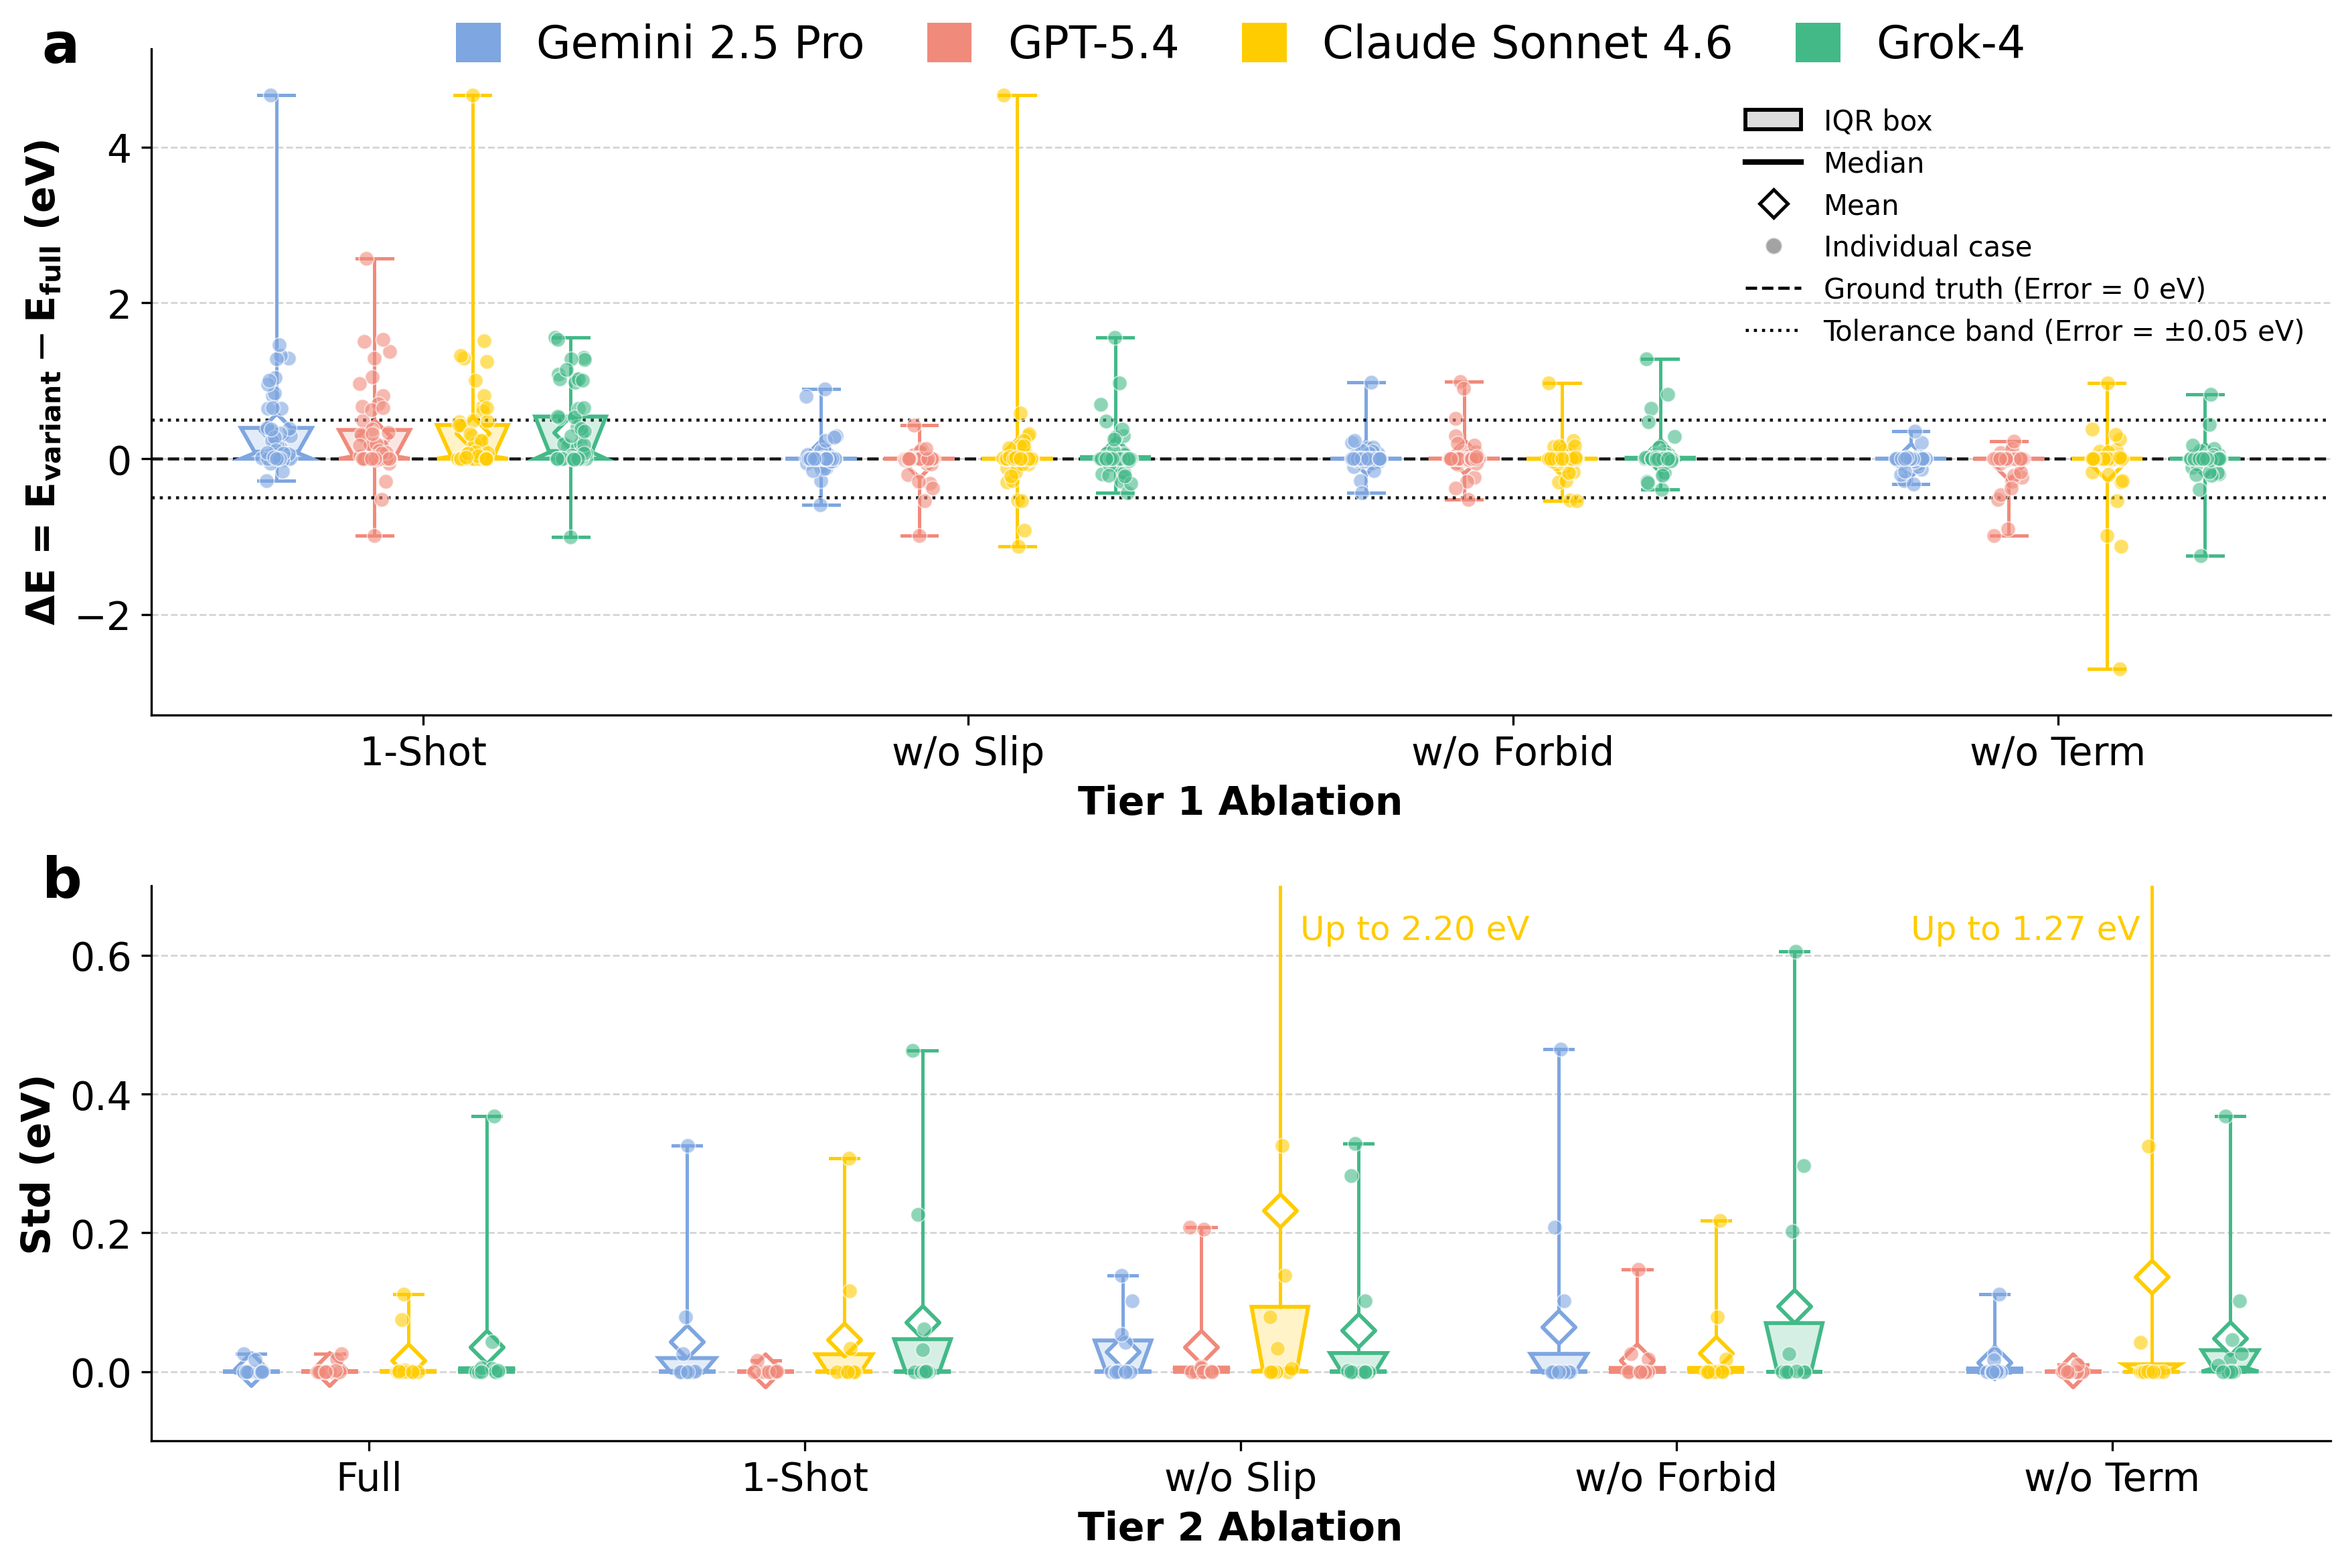
\includegraphics[width=0.95\linewidth]{images/figure4_ocd_2tier_overview.png}
  \caption{\textbf{Two-tier evaluation overview on OCD-GMAE62.} (a) Success rates by tier and variant: Full achieves $>$98\% success across both tiers, while 1-Shot drops to 89.5\% on Tier~1. (b) Energy degradation: mean 1-Shot penalty is $+0.329$~eV across Tier~1, with a wide distribution reflecting case-level heterogeneity. (c) Stability analysis on Tier~2 (12 cases, $N=3$, min-var selection): 79.2\% of Full-variant runs agree within 0.01~eV (72.9\% within 0.001~eV), with a thin stochastic tail where different runs explore distinct local minima.}
  \label{fig:ocd62-two-tier}
\end{figure}

\subsubsection{Tier~1: Full-matrix evaluation}

Full achieves 98.8\% success on Tier~1 (245/248), while 1-Shot drops to 89.5\% (222/248) (Figure~\ref{fig:ocd62-two-tier}a).
The three Full failures are concentrated on case~053 (K$_{20}$ + C([CH$_2$])O), where GPT-5.4, Gemini, and Grok-4 undergo natural adsorbate dissociation; Claude succeeds, confirming that the failure is a physical chemical event rather than a framework crash---the dissociating backends correctly identify surface instability, while Claude finds a bound configuration through an alternative site hypothesis.
All 33 failures across the ablation matrix are natural chemistry outcomes, with no API or implementation errors.

The aggregate 1-Shot penalty confirms that closed-loop iteration improves energy depth: mean $\Delta E = E_{\mathrm{1-Shot}} - E_{\mathrm{Full}} = +0.329$~eV (median 0.067~eV, Wilcoxon $p = 9.4 \times 10^{-24}$, $n=222$ paired cases), larger than the $+0.222$~eV penalty on CMU20 (Figure~\ref{fig:ocd62-two-tier}b).
However, this mean conceals extreme case-level heterogeneity that defines when closed-loop reasoning matters.
On complex, multi-element surfaces where no single high-symmetry site dominates, iterative feedback provides large gains: case~004 (Pt$_{16}$V$_{48}$ + [N]=O) improves by 1.05~eV, case~005 (As$_{48}$Hf$_{48}$Ni$_{48}$ + [NH$_2$]) by 0.82~eV, case~021 by 0.79~eV---precisely the regime where CMU20 slip rates reach 71--77\%.
On surfaces with a single dominant binding motif, iteration adds nothing: cases~007, 009, and 050 yield identical energies for Full and 1-Shot.
Conversely, on case~008 (Ga$_{12}$Pd$_{36}$ + [NH]), Full ($-7.48$~eV) is 0.99~eV \emph{worse} than 1-Shot ($-8.47$~eV): the LLM's first hypothesis is near-optimal, but the \texttt{FORBID} guardrail over-prunes the basin, trapping subsequent iterations in a shallower minimum.
The closed-loop advantage is thus conditional---largest when first-guess placement is unreliable, absent when a single dominant site exists, and occasionally negative when guardrails over-constrain a lucky guess.

\begin{table}[t]
\centering
\scriptsize
\caption{Complete five-variant ablation and cross-backend agreement on OCD-GMAE62 Tier~1 (62 cases $\times$ 4 backends). $\Delta E = E_{\mathrm{variant}} - E_{\mathrm{Full}}$; positive values indicate higher (worse) energy relative to Full. Range is the max--min spread across successful backends for each case. Success rates and mean $\Delta E$ are computed over successful runs only.}
\label{tab:ocd62-tier1-full}
\begin{tabular}{lrrrrrr}
\toprule
Variant & Successful & Success rate & Mean $\Delta E$ (eV) & Median $\Delta E$ (eV) & Mean 4-backend range (eV) & Within 0.01~eV \\
\midrule
Full      & 245 & 98.8\% & $+0.000$ & 0.000 & 0.183 & 24/61 \\
w/o Slip & 247 & 99.6\% & $+0.021$ & $0.000$ & 0.333 & 16/62 \\
w/o Forbid & 246 & 99.2\% & $+0.020$ & $0.000$ & 0.196 & 21/62 \\
w/o Term & 247 & 99.6\% & $-0.039$ & $0.000$ & 0.213 & 24/62 \\
1-Shot    & 222 & 89.5\% & $+0.329$ & 0.067 & 0.316 & 23/58 \\
\bottomrule
\end{tabular}
\end{table}

Aggregate statistics (Table~\ref{tab:ocd62-tier1-full}) show the ablated variants at near parity with Full (mean $|\Delta E| < 0.04$~eV), consistent with CMU20.
At the case level, however, ablated variants occasionally outperform Full: on case~007, w/o Slip reaches $-19.925$~eV vs.\ Full $-19.717$~eV; on case~008, Full is the worst of all five variants; on case~049, w/o Slip ($-8.628$~eV) outperforms Full ($-8.249$~eV).
These cases share a mechanism---when the first guess is already near-optimal, \texttt{FORBID} over-prunes---illustrating the reliability--exploration trade-off inherent to guardrail-based search.
Full also reduces the mean four-backend energy range to 0.183~eV from 0.316~eV under 1-Shot (1.73$\times$ reduction), a smaller compression than the 2.42$\times$ observed on CMU20, reflecting the greater difficulty of suppressing backend-specific biases on complex oxide and multi-element surfaces (Levene's test, $p < 0.01$).

Non-LLM baselines on OCD-GMAE62 confirm the breadth--depth trade-off established on CMU20: random placement ($N=20$) and heuristic enumeration (median 56 sites) both find lower energies than AdsMind Full at 5--25$\times$ more relaxations, but lack chemical-safety filters (see Supplementary Information for per-case data).
Under a fixed force field, energy depth is determined by sampling breadth, not reasoning strategy; AdsMind occupies the reliability-first, low-cost corner of this trade-off space.

\subsubsection{Tier~2: Stability audit}

Hosted LLM services are black-box stochastic systems; single-run energies risk reflecting lucky initialization rather than reproducible performance.
Tier~2 quantifies this by repeating 12 OCD-GMAE62 cases with $N=3$ independent runs, selected from $N=5$ by minimum-variance criterion with the seed-42 default run always retained.
Across 240 valid comparisons, 176 (73.3\%) agree within 0.01~eV and 165 (68.8\%) within 0.001~eV; the distribution is visualized in Figure~\ref{fig:ocd62-two-tier}c.
For the Full variant: 38/48 (79.2\%) within 0.01~eV (72.9\% within 0.001~eV), median run-to-run range $<$0.001~eV, mean range 0.034~eV.
The dominant pattern is exact reproducibility: 72.9\% of Full runs converge to identical energies across independent trials, reflecting the closed-loop architecture's ability to drive heterogeneous LLM planners toward consistent physical solutions.
A thin stochastic tail ($\sim$21\%) exhibits genuine multi-basin exploration driven by LLM nondeterminism, with energy differences up to 0.5--1.0~eV; this residual variance means single-run energies should not be over-interpreted even under the min-var selection protocol.

Stability is architecture-dependent, not backend-dependent.
Ranking variants by median run-to-run range yields: Full $\approx$ w/o Slip ($<$0.001~eV) $<$ w/o Forbid $\approx$ w/o Term ($<$0.01~eV) $<$ 1-Shot (0.015~eV).
Removing individual mechanisms modestly increases variance (they are partially redundant suppressors), while removing all feedback increases the median range by over an order of magnitude.
This ranking holds across all four backends, confirming that iterative feedback---not LLM choice---is the primary driver of reproducibility.

Synthesizing across Tier~1 and Tier~2, OCD-GMAE62 defines the conditions under which AdsMind's closed-loop architecture adds value.
On complex surfaces with multi-atom adsorbates, the closed loop provides both reliability (98.8\% vs.\ 89.5\%) and energy improvement (mean $+0.329$~eV) at $\sim$4 relaxations per case.
On simple surfaces with a single dominant site, 1-Shot matches Full and iteration adds nothing beyond reliability guarantees.
On rare edge cases (case~008), guardrails over-constrain a lucky first guess, making Full worse by up to $\sim$1~eV.
For autonomous workflows where failure is costly and every relaxation is expensive, the 98.8\% success rate and $\sim$4-relaxation budget are decisive; for applications tolerating 10\% failure with 20--100 relaxations per case, brute-force enumeration will find deeper energies.
The closed-loop architecture is a purpose-built tool for the reliability-first corner of this trade-off space---not a universal replacement for exhaustive search.

While the benchmarking above establishes AdsMind's reliability--cost profile under a fixed MLFF, a practical question remains: do the configurations identified by these search strategies agree with established DFT ground truth, and what are the consequences for experimental catalyst discovery? We address both questions below.

\subsection{DFT Verification and Comparison}

\subsubsection{DFT Benchmark against VASP Reference}

To benchmark the physical fidelity of adsorption energies predicted by the LLM-driven search strategies against an established ground truth, we compared AdsMind against DFT reference calculations (VASP/PBE, Section~\ref{sec:dft_reference}), alongside the original Adsorb-Agent results (EquiformerV2 backend) from Ref.~\citenum{ock2026adsorbagent}, on six representative CMU20 systems (cases~1, 2, 3, 4, 9, and~10). These systems cover three surface compositions (Mo$_3$Pd(111), CuPd$_3$(111), Pt(111)/(100)) and three adsorbates (H, NNH, OH), and were selected for their high practical relevance: Mo$_3$Pd is an experimentally established catalyst for both hydrogen evolution (HER) and nitrogen reduction (NRR)~\cite{zhou2023enhanced}, while Pt serves as the benchmark noble-metal catalyst for HER and oxygen evolution (OER)~\cite{cheng2016platinum}. Results are shown in Figure~\ref{fig:vasp_validation}.

\begin{figure}[t]
    \centering
    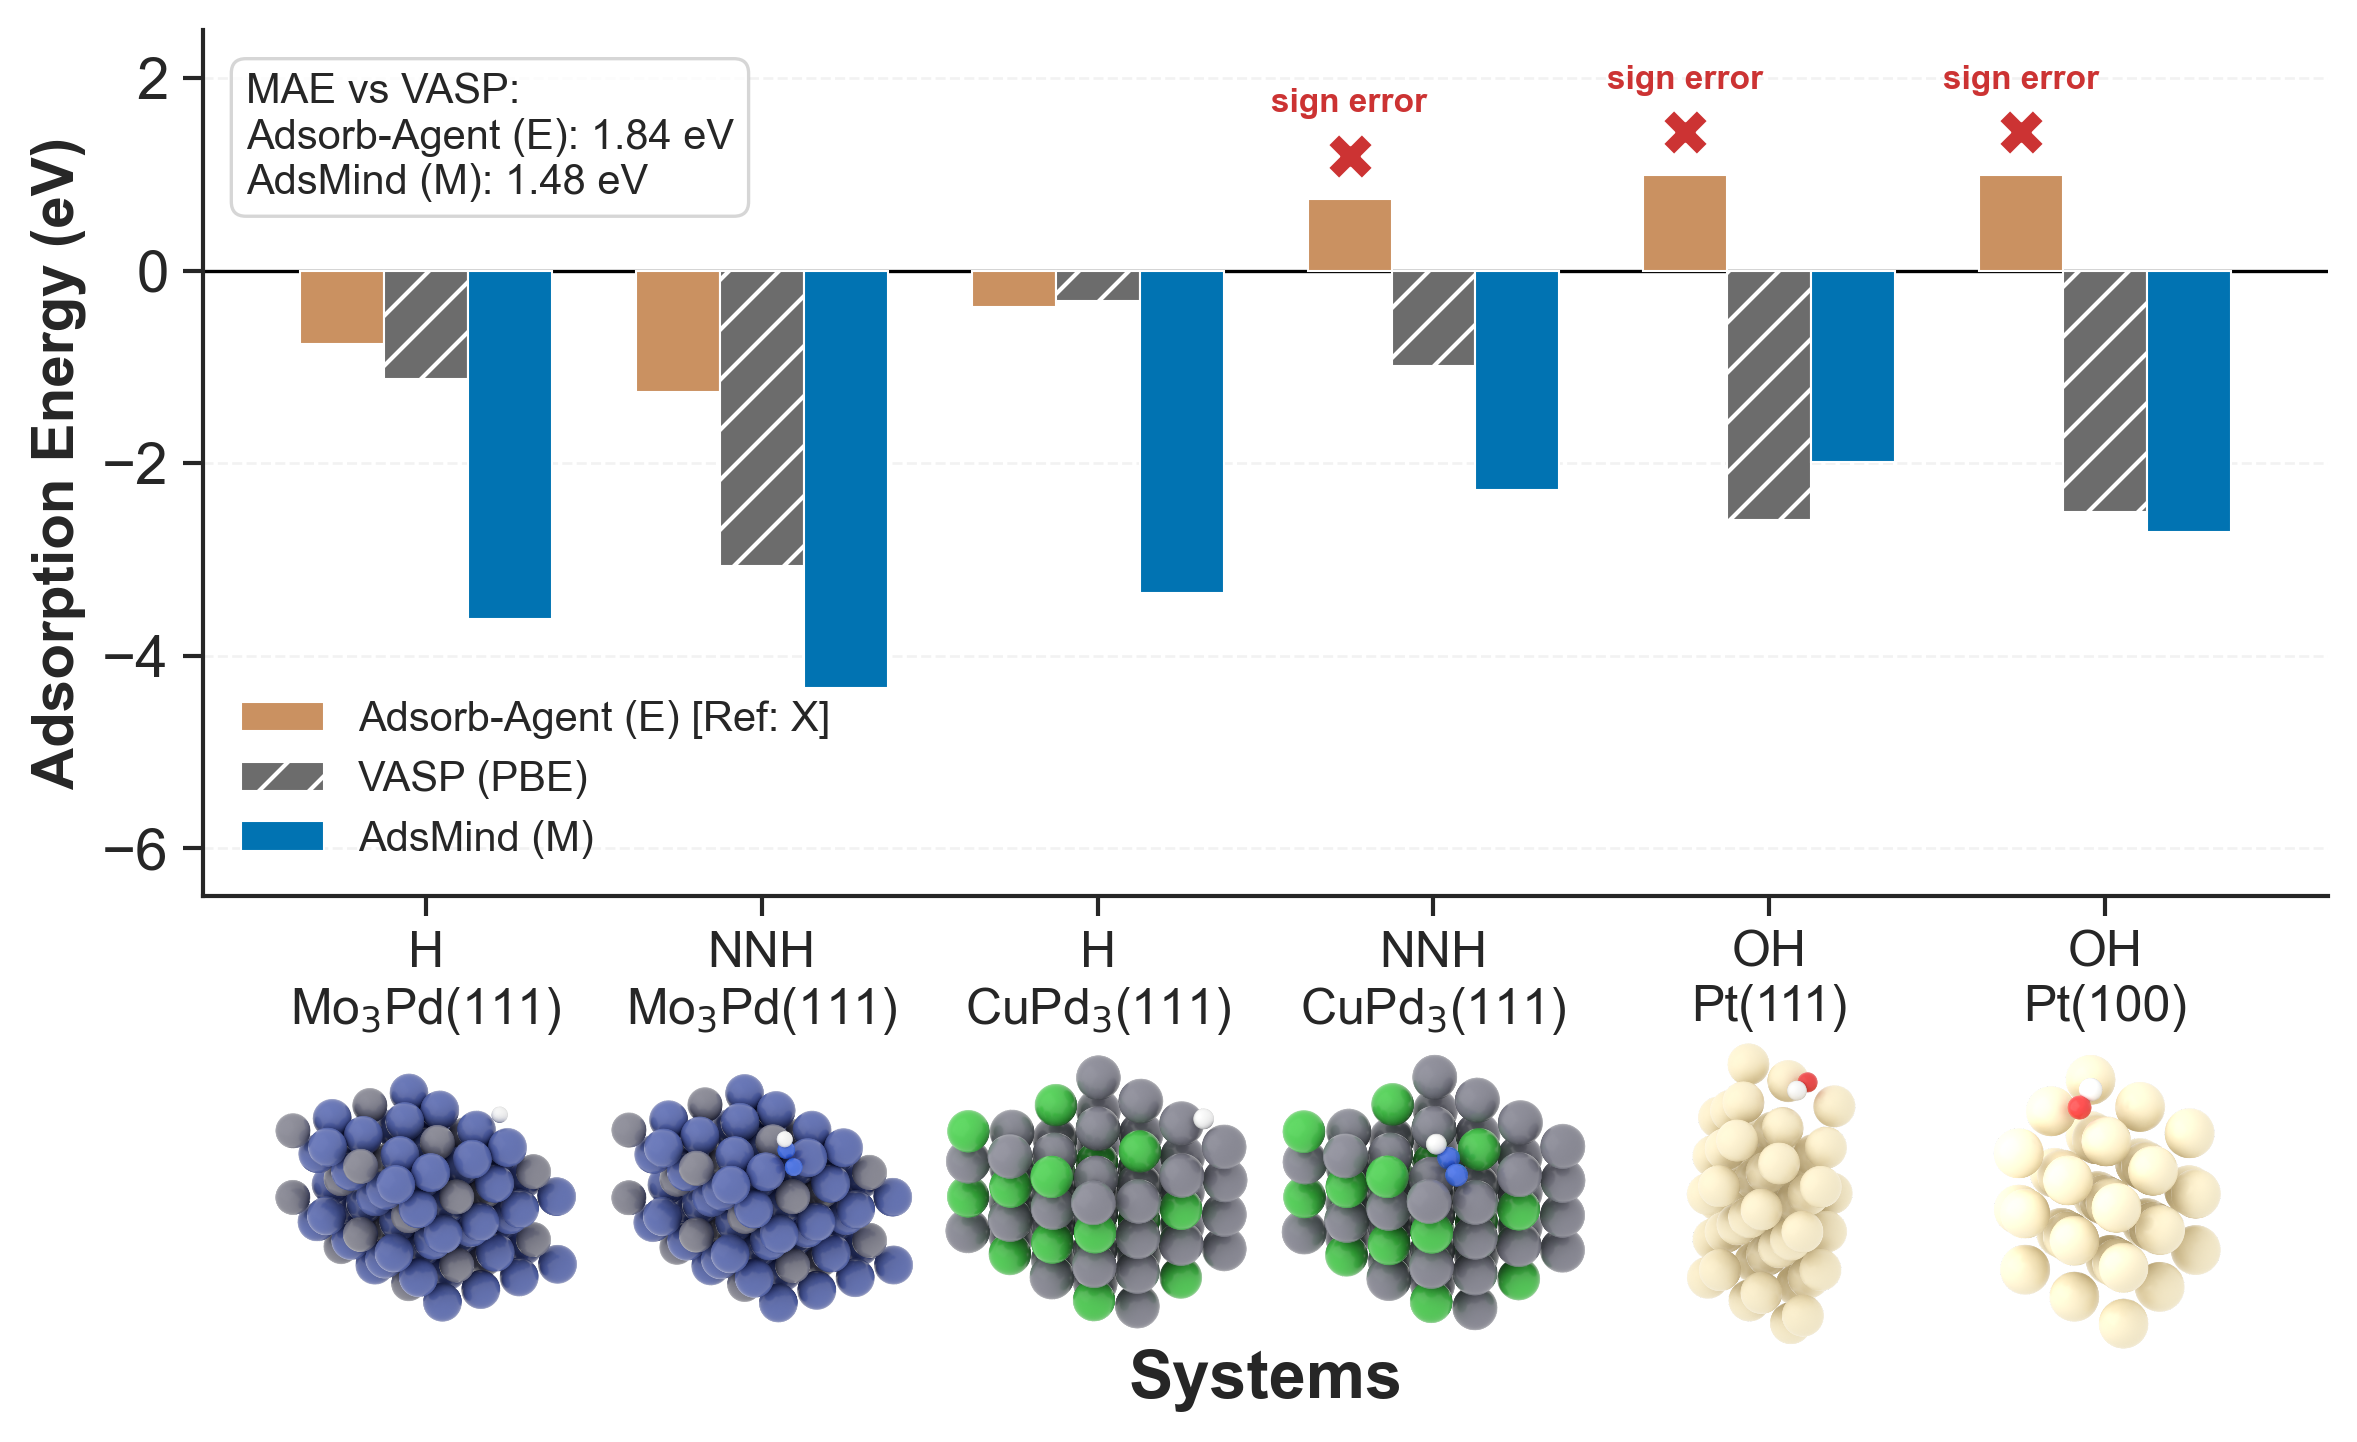
\includegraphics[width=0.95\linewidth]{images/figure5_vasp_validation.png}
    \caption{\textbf{DFT validation on six representative CMU20 systems.} Grouped bar chart comparing adsorption energies (eV) from Adsorb-Agent (original EquiformerV2 results~\cite{ock2026adsorbagent}), VASP (PBE), and AdsMind (MACE-MP-0 small). AdsMind preserves the correct sign of adsorption energy across all six systems (MAE 1.48~eV); Adsorb-Agent exhibits qualitative sign errors on OH--Pt and NNH--CuPd$_3$ systems (MAE 1.84~eV).}
    \label{fig:vasp_validation}
\end{figure}

The comparison reveals a sharp contrast between the two strategies (Figure~\ref{fig:vasp_validation}).
Adsorb-Agent exhibits large systematic deviations from VASP, with a mean absolute error (MAE) of 1.84~eV and a maximum deviation exceeding 3.5~eV on Pt(111)--OH.
Critically, the open-loop method produces qualitative sign errors on structurally complex adsorbates: it predicts endothermic binding for OH on both Pt(111) and Pt(100) ($+0.99$~eV for both), while VASP yields strongly exothermic values ($-2.59$~eV and $-2.51$~eV, respectively); similarly, NNH on CuPd$_3$(111) is predicted as endothermic ($+0.745$~eV vs.\ VASP $-0.996$~eV).
These sign errors would incorrectly disqualify Pt and CuPd$_3$ as candidate catalysts---a false negative with severe consequences for screening pipelines.
For simple adsorbates such as atomic H, Adsorb-Agent achieves reasonable accuracy (maximum error $\le 0.36$~eV), but structurally complex adsorbates drive its MAE to 1.84~eV with a high rate of sign errors.

AdsMind, by contrast, achieves better agreement with VASP (MAE 1.48~eV) and 100\% correctness in predicting the sign of adsorption energy across all six systems.
Although AdsMind quantitatively overbinds certain Mo$_3$Pd configurations---consistent with the known tendency of MACE-MP-0 on early-transition-metal alloys---it correctly identifies exothermic binding in every case, including the Pt--OH and CuPd$_3$--NNH systems where the open-loop method fails.
No sign errors are observed under either architecture on atomically simple H-on-metal systems, confirming that sign-correctness failures are specific to structurally complex adsorbates probed by open-loop exploration.

This contrast reframes the architecture comparison: whereas Sections~3.2--3.4 established AdsMind's advantage in reliability and cost, the DFT benchmark reveals a deeper qualitative failure mode of open-loop search---sign errors on complex adsorbates---that closed-loop iteration systematically prevents.
AdsMind converges on sign-correct configurations for all six systems with $\sim$4 relaxations per case, while Adsorb-Agent produces sign errors on 3 of the 4 complex-adsorbate systems despite $\sim$21 relaxations on successful cases.

\subsubsection{Implications for Computational Catalyst Discovery}

The DFT results carry significant practical implications.
Full VASP relaxation of a single adsorbate--surface system with the present parameter settings typically requires $>$48~hours of wall-clock time; initiating such an expensive calculation from a qualitatively wrong initial configuration---endothermic when the true binding is exothermic, as Adsorb-Agent produces for Pt--OH---would waste computational resources on configurations that should never have entered the DFT queue.
AdsMind's combination of 100\% sign-correctness and $\sim$4 relaxations per case eliminates this failure mode at negligible MLFF cost, delivering a reliable pre-screening filter before committing DFT hours.

For a high-throughput pipeline evaluating 1{,}000 candidate materials, AdsMind's $\sim$4{,}000 MLFF relaxations ($\sim$200 core-hours) correctly identify which candidates bind exothermically, versus $\sim$50{,}000 DFT-hours for exhaustive first-principles validation.
By eliminating endothermic candidates at the MLFF stage, this tiered workflow concentrates DFT resources on the most promising subset.

This architecture positions AdsMind as the first computational stage in an integrated discovery pipeline: high-throughput MLFF pre-screening identifies sign-correct, exothermic candidates; targeted DFT validation refines the energetics; and experimental synthesis focuses on materials whose computational signatures are qualitatively reliable.
For complex reaction intermediates---such as NNH in nitrogen reduction and OOH in oxygen evolution---traditional quantum-chemical relaxation is more than an order of magnitude ($>20\times$) slower than MLFF-based pre-screening.
By shifting the bottleneck from expensive first-principles relaxation to rapid MLFF pre-screening with sign-correctness guarantees, this workflow addresses the long-standing reliance on empirical intuition in catalyst design and accelerates the development of efficient, stable, and low-cost catalytic materials for sustainable energy technologies.

These results establish DFT-validated sign-correctness as a property of the closed-loop architecture on the six tested systems, with the open-loop baseline exhibiting qualitative sign errors on complex adsorbates. Broader validation across additional surface compositions, adsorbate classes, and against experimental reference data is pursued in ongoing work.